\documentclass[11pt,a4paper,oneside]{report}
\usepackage[ngerman,english]{babel}
% \usepackage{url} or \usepackage{hyperref}
\usepackage[utf8]{inputenc} % Displays German 'Umlaute' correctly. Also some workaround, see Bibliography Management#BibTeX in wikibooks
\usepackage{graphicx}

\setcounter{secnumdepth}{3}
\setcounter{tocdepth}{5}
\renewcommand\abstractname{Abstract}

\begin{document}

\begin{titlepage}
	\centering
	% \includegraphics[width=0.15\textwidth]{example-image-1x1}\par\vspace{1cm}
	{\scshape\LARGE
		Hochschule der Medien
	\par}
	\vspace{1cm}
	{\scshape\Large
		Bachelorarbeit
	\par}
	\vspace{1.5cm}
	{\huge\bfseries
		Sicherheitsbetrachtungen von Applikations-Containersystemen in Cloud-Infrastukturen am Beispiel Docker
	\par}
	\vspace{2cm}
	{\Large\itshape
		Moritz Hoffmann
	\par}
	\vspace{0.5cm}
	{\Large
		Studiengang: Mobile Medien\\
		Matrikelnummer: 26135\\
		E-Mail: \texttt{mh203@hdm-stuttgart.de}
	\par}
	\vspace{1.5cm}
	{\Large Dezember 2015\par}
	% Bottom of the page
	\vfill
	{\Large
		\emph{Erstbetreuer:}\hfill\emph{Zweitbetreuer:}\\
		Prof. Dr. Joachim Charzinski\hfill Patrick Fröger\\
		Hochschule der Medien\hfill ITI/GN, Daimler AG
	\par}

\end{titlepage}


\title{Sicherheitsbetrachtungen von Applikations-Containersystemen in Cloud-Infrastukturen am Beispiel Docker}
\author{Moritz Hoffmann\\
  Studiengang Mobile Medien,\\
  Hochschule der Medien\\
  \texttt{mh203@hdm-stuttgart.de}}
\date{Dezember 2015}
% \date{\today}
\maketitle




% \linespread{1.3}            % 1.5x line spacing
% \linespread{1.6}            % Double line spacing
% \hfill test                 % insert horizontal stretched space
% \vfill test                 % insert vertical stretched space
% ,,German quotation marks``  % deutsche Anfuehrungszeichen

% this is a comment
Hallo %\cite{myquote1}
One more line %\cite[S.2]{myquote1,myquote2}
jooooo \cite{Senn2009}

\begin{figure}[h] % with [p], images is displayed on own page
    \centering
    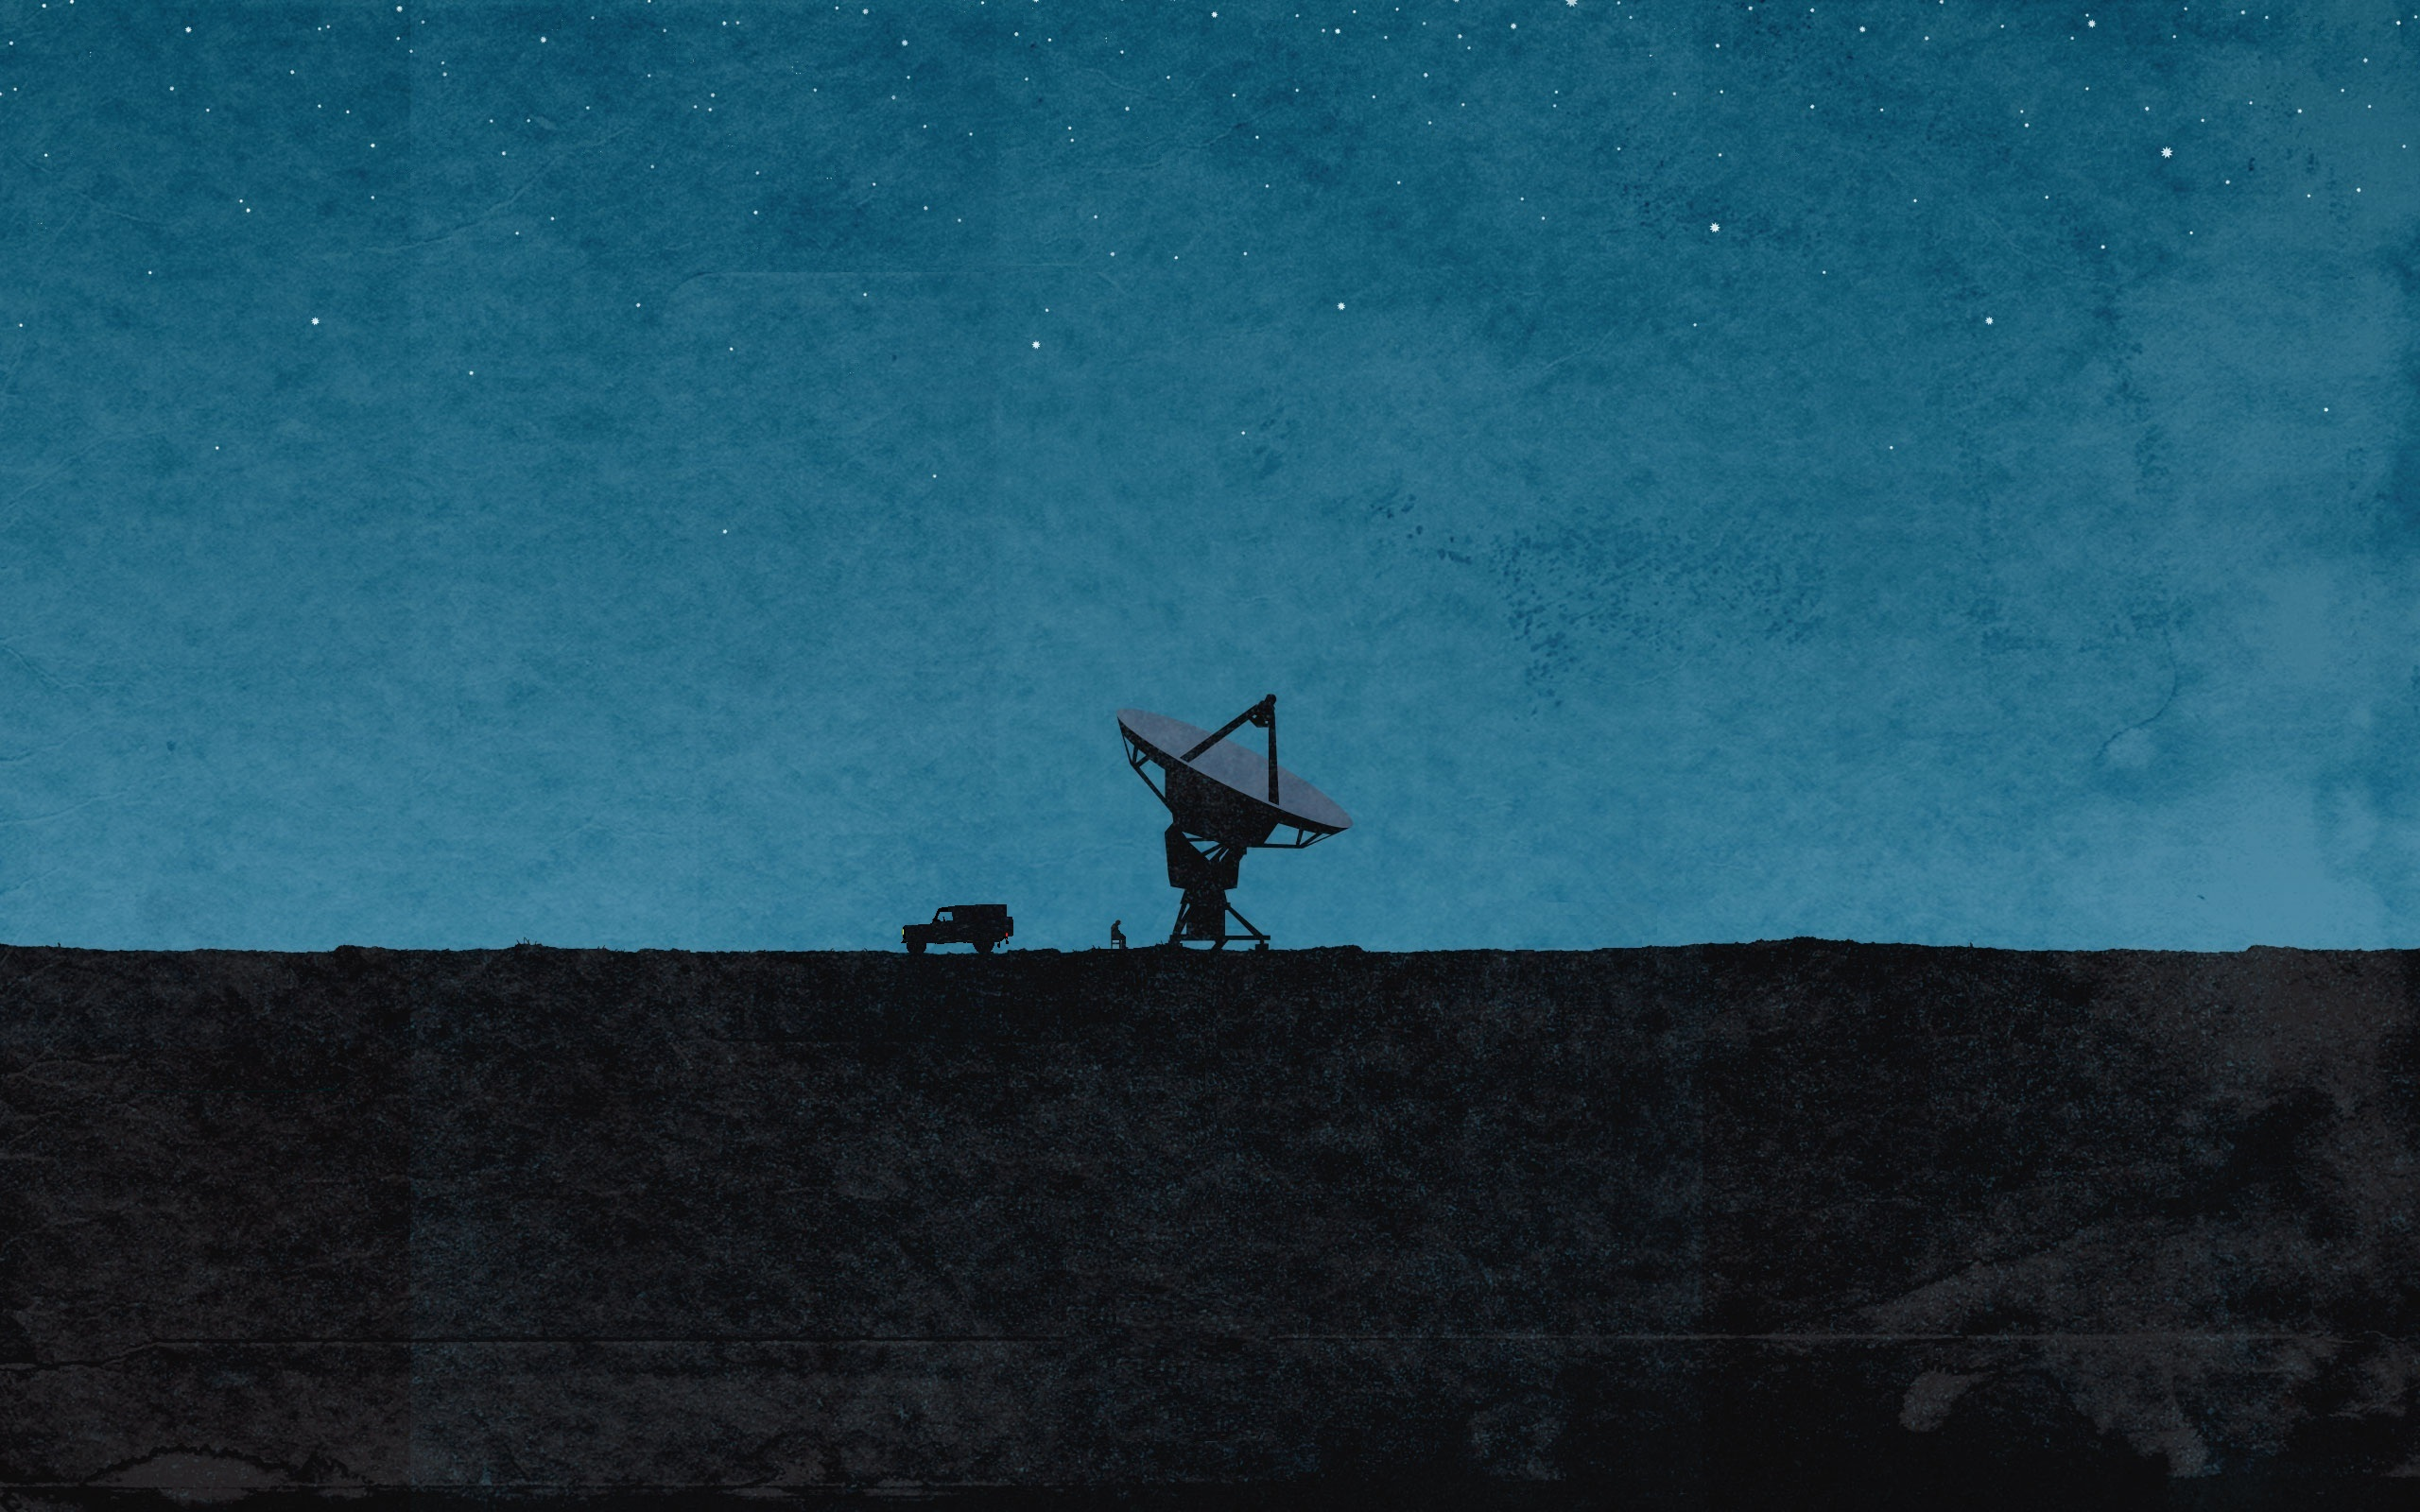
\includegraphics[width=0.9\textwidth]{./images/image.jpg}
    \caption{Awesome Image}
    \label{fig:awesome_image}
\end{figure}

lkasjdflkj asldkjf lasjkdflkadsjf ladksjflkjslkdjf    dslfjklaks df a sdfjaldsfj  ladksjf lkjlakjsd f asdf aljsdflkjasldfjalsdfj l adskjflj d f dslkfjalksdjf sd fljsdfkjsld f

\emph{dieser text ist kursiv}

asdfasdfasdfasdlkvalrkgjval  asdkfj  sldkfjlsdjfa adaher is kes ji lkaskdj ladskj a ldksfjll aldkfj lkj afsdlfkjl alsdkf jaldskfj la sdflaldsflas df sadfl sf

\texttt{das hier ist monotype}


\chapter{Kapitel Einfuehrung}
\section{Sektion bla}
\subsection{Subsektion blabla}
\subsubsection{Subsubsektion blablabla}
\paragraph{Paragraph soundso}
\subparagraph{SubParagraph soundso}

% Abstract
\begin{abstract}
...
\end{abstract}

% Table of Contents
\tableofcontents

% Abbildungsverzeichnis
\listoffigures

% Tabellenverzeichnis
\listoftables

% Anhang
\appendix

% Bibliography
\bibliographystyle{plain}
\bibliography{test} % specify name of bibfile

\end{document}
